\section{Experiments}\label{sec:exp}

\subsection{What is measured, and on what}

The detector is Grounding DINO \citep{liu2024grounding} with the public Swin-T
checkpoint, used exactly as distributed. Every image is queried with the phrases of the
categories that are annotated in it, once per wording, so that the five runs of an image
differ in nothing but the text. COCO contributes \NIMAGES{} images and 80 categories, which
the five wordings turn into \NPHRS{} distinct query phrases; the extraction takes about a
second per image for all five runs together, which is the cost of the measurement rather
than of the method.

A calibrator sees only cached \emph{(logit, phrase, label)} triples: it never touches an
image and never runs the detector. PhC accordingly fits on \FITROWS{} rows in seconds, and
adds 68 parameters to a 172\,M-parameter model.

\subsection{The wording moves the score}\label{sec:exp-measure}

Table~\ref{tab:setup} and Fig.~\ref{fig:word} report the measurement of
Section~\ref{sec:task}. The five rows are the same images, the same weights, the same
post-processing and the same category; the only difference is the sentence the user typed.

\begin{table}[t]
\caption{The five wordings on the same images with the same weights. A row is one phrasing; nothing but the text query changes between rows. ``Band'' is $p\in[0.3,0.9)$ of the uncalibrated score.}
\label{tab:setup}
\begin{tabular*}{\textwidth}{@{\extracolsep{\fill}}lrrrrrr@{}}
\toprule
Wording & detections & per image & positive rate & AP & share in band & ECE \\
\midrule
bare               & 1{,}063{,}949 & 215 & 3.2\% & 0.7770 & 4.3\% & 0.0500 \\
article            & 1{,}155{,}657 & 233 & 2.8\% & 0.7430 & 2.0\% & 0.0602 \\
photo              & 1{,}170{,}394 & 236 & 2.6\% & 0.4622 & 1.9\% & 0.0596 \\
image              & 1{,}169{,}850 & 236 & 2.7\% & 0.5020 & 2.2\% & 0.0512 \\
plural             & 1{,}133{,}371 & 229 & 3.0\% & 0.7217 & 2.6\% & 0.0474 \\
\bottomrule
\end{tabular*}
\end{table}


\begin{figure}[t]
\centering
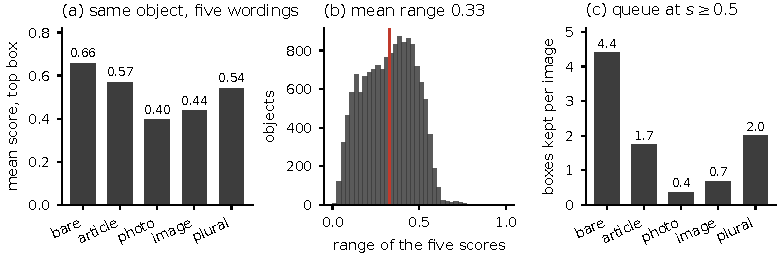
\includegraphics[width=\textwidth]{fig/fig1_wording.pdf}
\caption{The same objects, five wordings. (a) Mean score of the box the detector is most
confident about for an object, per wording. (b) Distribution over \NGROUPS{} objects of the
range of those five scores; the line is the mean. (c) How many boxes survive a fixed score cut of $0.5$, per
image: the queue a reviewer would be handed under a default threshold.}
\label{fig:word}
\end{figure}

Two sentences that name the same category do not produce the same number. The mean score
of the top box for an object is \SCBARE{} under the bare name, \SCART{} with an article,
\SCPHOTO{} under ``a photo of a'', \SCIMG{} under ``an image of a'' and \SCPLUR{} in the
plural: the five averages span a quarter of the scale, and the range within an object
(\SPREADPTS{} below) is wider still. Per object the range
of the five scores averages \SPREADPTS{} (median \SPREADMED), exceeds $0.1$ for \SPREADFRAC{}
of the \NGROUPS{} objects we can measure, and is \SPREADPOS{} even on the objects that all
five runs get right, where by construction there is nothing but the score to disagree
about. The disagreement is not confined to the score: the five runs agree on whether the
top box is correct at all for only \AGREE{} of the objects.

The consequence at a fixed threshold is immediate. A default cut of $0.5$ keeps
\BIGRATIO{} times as many boxes under one wording as under another
(Fig.~\ref{fig:word}c), so a reviewer who sets a threshold by eye under one phrasing has
set a different threshold under the next.

Average precision moves as well, from \APMIN{} to \APMAX{} (\APGAP). Part of that is
mechanical, because the score floor and the per-pair cap of Section~\ref{sec:task} discard
different boxes in different runs, so the five runs do not offer the same candidates. The
rest is not mechanical: among the boxes that survive, the phrasing also changes their
order, which is the part no post-hoc map can repair
(Proposition~\ref{prop:mono}). Either way the practical statement is the same one: with a
fixed capacity budget the detector returns a different amount of usable output depending
on how the user phrased the request.

\subsection{Calibrating the band}\label{sec:exp-calib}

Table~\ref{tab:main} fits each calibrator on half the images and evaluates on the other
half, inside each wording run, and averages over the five runs.

\begin{table}[t]
\caption{Calibration on the COCO half the calibrator never saw. Metrics are computed inside each wording run and averaged over the five runs. ``Band'' restricts to $p\in[0.3,0.9)$ of the uncalibrated score of that run. Lower is better except AP.}
\label{tab:main}
\begin{tabular*}{\textwidth}{@{\extracolsep{\fill}}lrrrrr@{}}
\toprule
Method & band ECE & band Brier & ECE & Brier & AP \\
\midrule
uncalibrated                       & 0.1800 & 0.2287 & 0.0536 & 0.0199 & 0.6395 \\
temperature scaling                & 0.2123 & 0.2421 & 0.0087 & 0.0173 & 0.6395 \\
vector scaling                     & 0.0812 & 0.1849 & 0.0051 & 0.0158 & 0.6395 \\
isotonic regression                & 0.1246 & 0.2428 & 0.0076 & 0.0180 & 0.5236 \\
per-wording temperature            & 0.2108 & 0.2418 & 0.0079 & 0.0172 & 0.6395 \\
PhC (phrase, linear)               & 0.0597 & 0.1817 & 0.0040 & 0.0157 & 0.6395 \\
PhC (phrase, linear, band-weighted) & 0.0324 & 0.1754 & 0.0068 & 0.0157 & 0.6395 \\
PhC+category                       & \textbf{0.0322} & \textbf{0.1729} & 0.0065 & 0.0155 & 0.6395 \\
\bottomrule
\end{tabular*}
\end{table}


\begin{figure}[t]
\centering
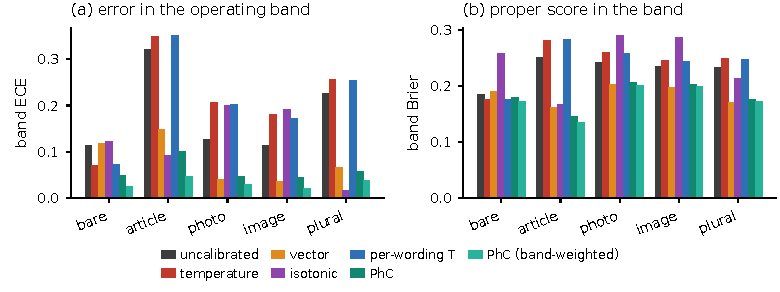
\includegraphics[width=\textwidth]{fig/fig2_calib.pdf}
\caption{Band ECE (a) and band Brier (b) per wording, for the calibrators of
Table~\ref{tab:main} except the per-category variant, on the half of COCO the calibrator did
not see. The band is fixed by the uncalibrated score of each run,
so all bars of a group are computed on the same detections.}
\label{fig:calib}
\end{figure}

Prompt-conditioned calibration reduces the error in the operating band from \BANDID{}
[\BANDIDCI] to \BANDPHC{} [\BANDPHCCI], a factor of \FACTOR, and the proper score on the same
detections from \BANDBSID{} to \BANDBS. The brackets are 95\% intervals from \BOOTN{}
resamples of the test images, which is the right unit: the rows of one image are strongly
correlated, so a detection-level interval would be far too narrow. The reduction itself is
\DROP{} [\DROPCD]. The two scalar baselines do not merely fail to help, they hurt:
temperature scaling raises the band error to \BANDTEMP{} and a separate temperature per
wording, the strongest scalar model available once the wording is known, to a level
indistinguishable from it. This is the point of Section~\ref{sec:method}: the two
parameters are fitted to an objective dominated by the $97\%$ of detections outside the
band, and the band inherits whatever is left over.

Two rows deserve comment. Vector scaling reaches \BANDVEC{} [\BANDVECCI], an interval that
does not overlap PhC's, because a per-category scale and bias absorb much of what the phrase
does --- at the price of a table indexed by category, which Section~\ref{sec:exp-transfer}
shows is exactly what does not survive a new vocabulary. Isotonic regression reaches
\BANDISO{} and pays for it with \APISO{} against \APID: it is free to reorder a run, and it
does. Every method in the table that \emph{is} monotone within a run reports the same AP as
doing nothing, \APID, which is Proposition~\ref{prop:mono} measured rather than assumed.

The last row adds a term indexed by category to PhC and is the best in both error columns, by
\BANDCATF{} against \BANDPHCF{}: a difference in the fourth decimal, well inside the interval
above. Once the descriptor of the phrase is in the map, the category table has nothing left to
supply on the corpus it was fitted on; on a corpus whose categories are new it has nothing to
look up at all (Section~\ref{sec:exp-transfer}). We therefore carry PhC without the table, and
the bold entries of Table~\ref{tab:main} are simply the minima of their columns, not the
configuration we recommend.

\subsection{A wording the calibrator has not seen}\label{sec:exp-heldout}

A practitioner can enumerate the phrasings they use; they cannot enumerate the ones their
users will type. Table~\ref{tab:heldout} therefore fits on bare, article and photo, and
deploys on ``an image of a'' and the plural, which the calibrator has never seen. The
uncalibrated row is the reference: a calibrator is only useful here if it beats doing
nothing on a wording it was not fitted on.

\begin{table}[t]
\caption{Fitted on three wordings (bare, article, photo) and deployed on the two it never saw. The uncalibrated row is the reference: a calibrator is only useful here if it beats doing nothing on an unseen wording.}
\label{tab:heldout}
\begin{tabular*}{\textwidth}{@{\extracolsep{\fill}}lrrrr@{}}
\toprule
Method & \multicolumn{2}{c}{``an image of a''} & \multicolumn{2}{c}{plural} \\
\cmidrule(lr){2-3}\cmidrule(l){4-5}
 & band ECE & band Brier & band ECE & band Brier \\
\midrule
uncalibrated                       & 0.1128 & 0.2342 & 0.2257 & 0.2333 \\
temperature scaling                & 0.1847 & 0.2472 & 0.2580 & 0.2509 \\
vector scaling                     & 0.0144 & 0.2041 & 0.0818 & 0.1802 \\
isotonic regression                & 0.2187 & 0.2975 & 0.0424 & 0.2143 \\
per-wording temperature            & 0.1873 & 0.2480 & 0.2593 & 0.2518 \\
PhC (phrase, linear)               & 0.0653 & 0.2130 & 0.2342 & 0.2378 \\
PhC (phrase, linear, band-weighted) & 0.0577 & 0.2142 & 0.2225 & 0.2360 \\
PhC+category                       & 0.0217 & 0.2023 & 0.2289 & 0.2415 \\
\bottomrule
\end{tabular*}
\end{table}


On ``an image of a'' PhC brings the band error from \HELDID{} down to \HELDBAND{} with no
category table, and to \HELDPHC{} with one. On the plural neither helps: \HELDBANDPL{} and
\HELDPLURAL{} against \HELDPLURALID{} for doing nothing.

Vector scaling is much better than any of them on both unseen wordings, \HELDVECIMG{} and
\HELDVEC{}, and the reason is instructive. Its table is indexed by category, and the
categories here are the ones it was fitted on --- only the sentence is new, so the entry
for a category still supplies the category-specific part of the offset while the shared scale
absorbs the wording. Section~\ref{sec:exp-transfer} shows the same table failing completely
when the categories are the new part. The two experiments therefore locate the difficulty on
two different axes: a per-category table generalises along wordings and not along
vocabularies, a phrase descriptor generalises along vocabularies and only partly along
wordings. PhC leads on COCO because there both axes are inside its training set; a wording it
has not seen is the case where it falls behind a table.

Isotonic regression reaches \HELDISO{} on the plural, the best number in the table, and pays
\HELDISOAP{} against \APID{} for it: it is allowed to reorder the run, which is the freedom the
other rows do not have (Proposition~\ref{prop:mono}).

We report this because it delimits the claim: PhC is not a substitute for a category table
when the categories are known and the wording is not. What it substitutes for is the category
table itself, and that is the setting in which an open-vocabulary detector is actually used.

\subsection{What a threshold is worth}\label{sec:exp-fdr}

A calibrated score is not yet a decision. Table~\ref{tab:fdr} compares three ways to end
up with a threshold at target $\alpha=\ALPHAMAIN$, and reports for each the false
discovery rate of the \emph{worst} of the five wordings, which is what a guarantee has to
cover.

\begin{table}[t]
\caption{Three ways to choose a threshold at target $\alpha=0.30$, fitted on the calibration half and measured on the other. ``Pooled'' is one $\hat\lambda$ from the calibration rows of all five wordings, ``worst-case'' is the most conservative of the five per-wording $\hat\lambda$, and ``per-wording'' selects inside each wording. Each cell pair gives the false discovery rate of the \emph{worst} of the five wordings and the number of boxes kept across all five. The worst wording is the one that a guarantee has to cover.}
\label{tab:fdr}
\begin{tabular*}{\textwidth}{@{\extracolsep{\fill}}lrrrrrr@{}}
\toprule
 & \multicolumn{2}{c}{pooled $\hat\lambda$} & \multicolumn{2}{c}{worst-case $\hat\lambda$} & \multicolumn{2}{c}{per-wording $\hat\lambda$} \\
\cmidrule(lr){2-3}\cmidrule(lr){4-5}\cmidrule(l){6-7}
Score & max FDR & kept & max FDR & kept & max FDR & kept \\
\midrule
uncalibrated & 0.406 & 57{,}824 & 0.310 & 44{,}163 & \textbf{0.310} & 59{,}442 \\
temperature scaling & 0.406 & 57{,}824 & 0.310 & 44{,}163 & \textbf{0.310} & 59{,}442 \\
vector scaling & 0.393 & 59{,}848 & 0.321 & 48{,}701 & 0.321 & 61{,}536 \\
PhC (phrase, linear) & \textbf{0.380} & 62{,}068 & \textbf{0.294} & 49{,}084 & 0.313 & 61{,}087 \\
\bottomrule
\end{tabular*}
\end{table}


\begin{figure}[t]
\centering
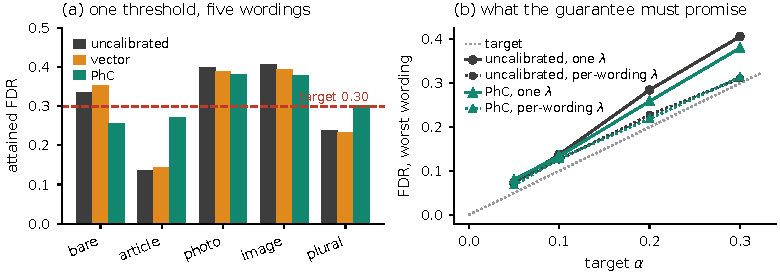
\includegraphics[width=\textwidth]{fig/fig3_fdr.pdf}
\caption{(a) False discovery rate actually attained under a single pooled threshold
calibrated at $\alpha=0.30$, per wording. (b) Attained FDR of the worst wording as the
target varies, for a single threshold and for one threshold per wording.}
\label{fig:fdr}
\end{figure}

The pooled threshold is the natural thing to ship and it does not work. Calibrated on the
mixed wordings at $\alpha=\ALPHAMAIN$, it delivers \FDRWORST{} on the wording that fares
worst --- an overshoot by a factor of \FDROVERSHOOT{} --- and Fig.~\ref{fig:fdr}a shows
the ordering of the five wordings, not a uniform bias that a better global calibration
could absorb.

The reason is Proposition~\ref{prop:mono} read backwards. The false discovery rate at a
shared threshold is set by the \emph{order} of the boxes within each run, and no monotone
map can change that order. Calibration moves the scale, so it can make scores comparable,
but it cannot make two wordings agree about which boxes are the good ones when they
already disagree. None of the five calibrators in Table~\ref{tab:main}, including PhC,
closes the gap; Fig.~\ref{fig:fdr}b shows the residual, and we report it as a negative
result because it is the one we did not expect.

What does hold is a threshold chosen to satisfy the constraint inside every wording
separately. Taking the strictest of the five per-wording thresholds needs no multiplicity
correction --- the maximum over strata is the simultaneous statement --- and its worst wording
lands at \FDRWCPHC{} for PhC and \FDRWCID{} for the uncalibrated score (Table~\ref{tab:fdr},
middle block), against a target of \ALPHAMAIN. That is an excess of one point, where the
pooled threshold is eleven points over, and it is the calibration-to-test gap of a finite
sample rather than a systematic overshoot: the threshold is fitted on one half and measured on
the other. It costs boxes, and
that cost is where calibration pays for itself, though not by much: relative to the pooled
threshold the guarantee costs \WCCOSTID{} of the kept boxes for the uncalibrated score and
\WCCOSTPHC{} for PhC, and at the same target PhC keeps \WCGAIN{} more boxes than the
uncalibrated score under the guarantee (\WCTOTALPHC{} against \WCTOTALID). A score whose
wordings agree more closely has a less binding worst case, so the gain is in the direction
we predicted, but a tenth of the coverage is a modest return and we do not want to sell it
as more.

\subsection{A vocabulary the calibrator has not seen}\label{sec:exp-transfer}

The last protocol is the one that separates a calibrator which has learned something about
phrases from one which has memorised categories. We fit on COCO and deploy on the LVIS v1.0
minival split without refitting anything: not the head, not the projection of the descriptor,
not a per-category table. The run covers the \NLVISIMG{} images of the split that carry an
annotated instance, \NLVISNDET{} detections over \NLVISCAT{} categories, none of which was
seen during fitting.

\IfFileExists{tables/tab_transfer.tex}{\begin{table}[t]
\caption{Fitted on COCO and deployed on the LVIS minival split without refitting anything, including the projection used by the phrase descriptor. None of the 1{,}203 LVIS categories was seen during fitting, so a calibrator with a table indexed by category has nothing to look up.}
\label{tab:transfer}
\begin{tabular*}{\textwidth}{@{\extracolsep{\fill}}lrrrr@{}}
\toprule
Method & band ECE & band Brier & ECE & AP \\
\midrule
uncalibrated                       & 0.1978 & 0.2352 & 0.0478 & 0.5771 \\
temperature scaling                & 0.2434 & 0.2520 & 0.0119 & 0.5771 \\
vector scaling                     & 0.2766 & 0.2734 & 0.0203 & 0.5771 \\
isotonic regression                & 0.1118 & 0.2349 & 0.0078 & 0.5093 \\
per-wording temperature            & 0.2423 & 0.2530 & 0.0118 & 0.5771 \\
PhC (phrase, linear)               & 0.1136 & 0.2015 & 0.0090 & 0.5771 \\
PhC (phrase, linear, band-weighted) & \textbf{0.0838} & 0.1936 & 0.0105 & 0.5771 \\
\bottomrule
\end{tabular*}
\end{table}
}{}

Band error on LVIS falls from \TRBANDID{} to \TRBANDPHC{}, a factor of \TRFACTOR, with AP
unchanged at \TRAPID. The phenomenon travels with the vocabulary as well: on a corpus with
1{,}203 categories the calibrator never saw, the same two wordings lead and trail as on COCO,
the bare name at \TRAPHI{} and ``a photo of a'' at \TRAPLO{}, a gap of \TRAPGAP. So the wording
matters because the score is a function of the text query, not because of anything specific to
the 80 COCO categories or to the way they are annotated.

The transfer is not uniform, and we report the uneven part. Under an indefinite article the
band error goes from \TRARTID{} to \TRARTPHC; under the bare name only from \TRBAREID{} to
\TRBAREPHC. Averaging over the five wordings would hide the failure: the bare name is the one
wording where the map does not close the gap, and the other four end between $0.030$ and
$0.080$. Bare is also the wording that moves most between the two corpora --- its band error is
\COCBARE{} on COCO and \TRBAREID{} on LVIS --- so part of what the descriptor has to extrapolate
is a property of the corpus rather than of the phrasing, and a linear head on text features
does not have the information to do it.

Vector scaling, the strongest baseline on COCO, reaches \TRBANDVEC{}: it has a scale and a
bias for \VECSEEN{} categories, none of which is present in LVIS, so every detection falls
back to the average of the fitted scales and the bias term is unavailable. That fallback is
worse than an uncalibrated score, and the reason is worth stating: a table indexed by a label
the deployment does not have does not merely fail to help, it actively mis-calibrates, because
the average of the per-category scales is not the scale the new vocabulary needs. Temperature
scaling, which has no table, lands at \TRBANDTEMP: worse than doing nothing, for the reason of
Section~\ref{sec:exp-calib} --- its single parameter serves the $97\%$ of detections outside
the band. A calibrator whose parameters are indexed by a label cannot be shipped to a
deployment that adds labels, which is what an open-vocabulary detector is for; a calibrator
with two global parameters cannot be shipped to a deployment whose wording changes either.

Isotonic regression is the other method here that carries no per-category table, and it does
transfer, to \TRBANDISO{}; it pays for that with AP, \TRAPISO{} against \TRAPID, which is the
price of a map that is free to reorder a run. PhC is the only one of the two that fixes the
band without touching the ranking, and on a vocabulary it has never seen it is the only
method in the table that improves the band at all.
